\chapter{软件变更冲突检测方法}
\label {chap_conflict}

本章中主要介绍软件变更冲突检测方法,包括具体的检测算法、相应的模块设计与实现等。

软件变更冲突检测主要用于对变更影响域之间是否发生冲突进行判定。本文中实现了简单的自动分析算法,通过判断变更影响域之间是否存在重叠来找到可能存在冲突的代码位置,并结合人工分析来完成最后的判定。

下面对该冲突检测方法和其对应模块的设计与实现进行具体的介绍。

\section{相关定义}

\label {conflict_define}

为了进行变更的冲突检测,需要知道什么是冲突。下文中的冲突都指语义冲突。

根据前文中的讨论,冲突实际上是指两个补丁所对应的不同变更集合之间存在某两条互斥的变更,即这两条变更的影响域发生了重叠。因此,冲突可以较形式化的定义如下,其中$\mathcal{C}$是某个版本的源代码文件中按照该语言的合法语法结构组织起来的代码,$\mathcal{P}$是变更集合,$impact$是求解影响域的函数:

\begin{definition}
	$conflict:\mathcal{P} \times \mathcal{P} \mapsto \{T,F\}$。$\forall p_i,p_j \subset \mathcal{P}$,如果$impact(p_i,v) \cap impact(p_j,v) \neq \varnothing$,那么就有$conflict(p_i,p_j) = T$,其中$v \subset \mathcal{C},i,j \subset \mathbb{N}$。即如果两个补丁分别对应的变更集合在某相同版本代码上的变更影响域之间产生了交集,那么就认为补丁间发生了冲突。
\end{definition}

综上所述,冲突是由于来自两个变更集合的某两条不同变更分别直接或间接的影响到了某个相同的语法结构而造成的,可见$conflict$函数描述了变更冲突检测的过程,它接受两个变更集合作为输入,并根据变更影响域计算其是否发生了冲突。

\section{分析方法}
\label {chap_conflict}

如前所述,冲突检测的过程即为$conflict$函数的具体实现。该分析过程将对比两个补丁间的变更影响域,通过判断变更影响域间是否重叠来检测其兼容性。

%该函数的实现可以定义如下:
%
%\begin{definition}
%		如果$\exists c_m \subset p_i, \exists c_n \subset p_j$,其中$c_m = change(structure_m),c_n = change(structure_n)$, $structure_m \subset Struct(v_k), structure_n \subset Struct(v_k), v_k \subset Code$,并且$i,j,k,m,n \subset \mathbb{N}$。
%		那么有$conflict(p_i,p_j) == true \iff (structure_m == structure_n) \lor (impact(p_i,v_k) \cap impact(p_j,v_k) \neq \varnothing)$,其中$p_i,p_j \subset Pat(v_k)$。
%\end{definition}

理论上来讲,由于重叠部分的代码显然是可能会发生冲突的,这种简单比对即可发现两个补丁间的兼容性问题。然而在具体实现中,受限于工具的精度,冲突检测方法往往不能达到理论上的准确度,而可能产生误报等情况。

如果重叠不存在,则补丁间的语义没有发生相互覆盖,因而不存在冲突。如果存在重叠,则对于重叠部分的代码而言,判断该位置是否确实发生了冲突需要人工分析的辅助。因为该代码位置的冲突判定与补丁的变更目的密切相关,而代码中无法直接获取到这种信息,因此只有依靠外界的干预来判定这部分代码是否确实存在冲突。

人工分析过程不仅需要知道哪部分代码出现了重叠,还需要知道是哪些变更影响到了这部分代码。因此冲突检测过程需要具有影响回溯的能力。由于变更影响域分析中的影响追踪系统会记录其分析过程的轨迹并存储程序语法结构间的影响关系,因此只需在冲突检测时对重叠部分的代码进行回溯即可追踪到具体的软件变更。

%可以看得出来,由于使用了更严格的冲突定义,我们的方法会造成一定的过高估计的结果。

该冲突检测过程可以参考算法\ref {algo_compatible}。

\begin{algorithm}[H]
	\caption{冲突检测}
	\label{algo_compatible}
	\begin{algorithmic}[1]
		\Require $s_1=impact(diff(v_2,v_1),v_2)$,$s_2=impact(diff(v_2,v_4),v_2)$
%		\\
%		\quad \quad $t_1=impact\_track(ia(v_2,v_1))$, $t_2=impact\_track(ia(v_2,v_4))$
		\Ensure $conflict(diff(v_2,v_1),diff(v_2,v_4))$
		\If{$s_1 = \varnothing \lor s_2 = \varnothing$}
		\State $result \gets False$
		\Else
		\State $s \gets s_1 \cap s_2$
		\If{$s = \varnothing$}
		\State $result \gets False$
		\Else				
		\State $result \gets Manual\_analysis(s_1, s_2)$
		\EndIf 
		\EndIf \\
		\Return $result$
	\end{algorithmic}
\end{algorithm}


\section{模块设计与实现}
\label {chap_mod}

冲突判定模块主要需要实现$conflict$函数的实际功能。目前根据上文所述的冲突检测算法实现了较为简单的自动分析过程,更精确的分析结果需要人工分析过程的辅助。

%\subsection{设计}
%
%在该模块的设计中,其输入输出过程可以描述如图\ref {com},输入输出的具体描述参见表\ref {com_io}。
%
%该模块的核心在于冲突分析算法\ref {algo_compatible},因此,根据算法中的描述,该模块可以设计如图\ref {des_com}所示。

考虑到该模块需要实现接受影响域分析模块的输入,并完成冲突检测的功能,该模块的核心任务应当包括:
\begin{itemize}
	\item 输入:读取软件变更影响域分析过程的输出,即该模块需要接受两个变更影响域作为其输入。
	\item 输出:找到可能发生冲突的代码位置,并输出其影响来源。即该模块需要输出变更影响域重叠处的代码位置(即可能发生冲突的位置)及其相关的影响关系。
	\item 影响域计算:存储读取的影响域信息,并计算其是否发生重叠。即该模块需要实现上文提出的冲突检测算法。
%	\item 冲突分析:根据影响域重叠,对找到的冲突进行影响回溯。
\end{itemize}


%因此,在冲突判定模块中,其流程可以设计如下:
%\begin{enumerate}
%	\item 读取影响域分析模块的结果
%	\item 计算是否发生影响域重叠
%	\item 对于发生了重叠现象的影响域,判定为可能发生冲突
%	\item 回溯冲突代码的影响来源并输出其影响关系
%	\item 根据得到的影响依赖关系进行人工分析,判定是否确实冲突
%\end{enumerate}

%\begin{figure}[H]
%	\centering
%	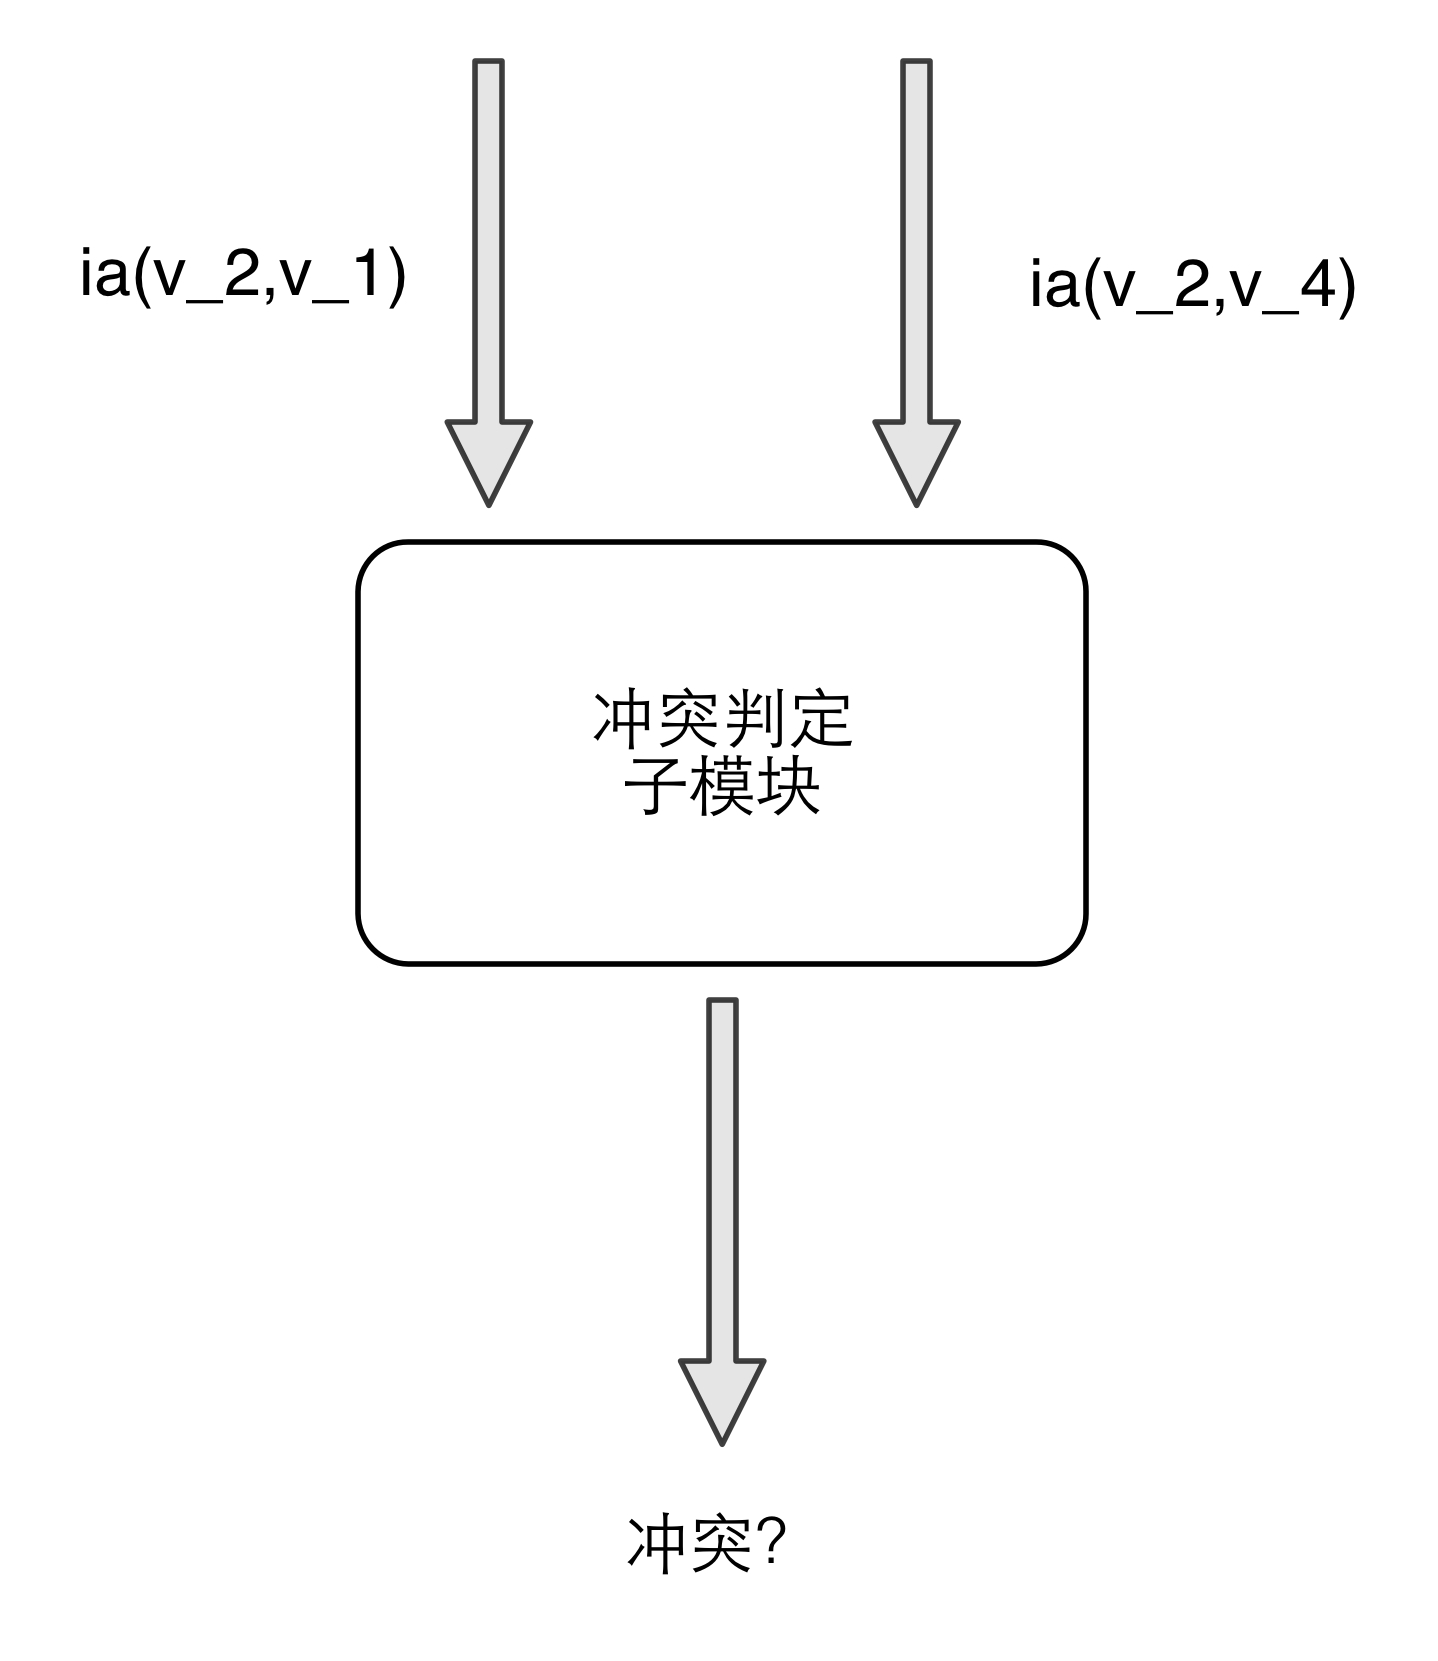
\includegraphics[height=.6\columnwidth]{chap03_com}
%	\caption {输入输出}
%	\label {com}	
%\end{figure}
%
%\begin{table}[H]
%	\caption{输入输出对照表}
%	\label{com_io}
%	\centering
%	\begin{tabular}{lc}
%		\toprule[1.5pt]
%		{\heiti 输入输出} & {\heiti 描述} \\\midrule[1pt]
%		$ia(v_2,v_1)$ & 影响域分析模块的输出,语义影响域 \\
%		$ia(v_2,v_4)$ & 影响域分析模块的输出,语义影响域 \\
%		输出 & 是否发生语义冲突\\
%		\bottomrule[1.5pt]
%	\end{tabular}
%\end{table}
%
%\begin{figure}[H]
%	\centering
%	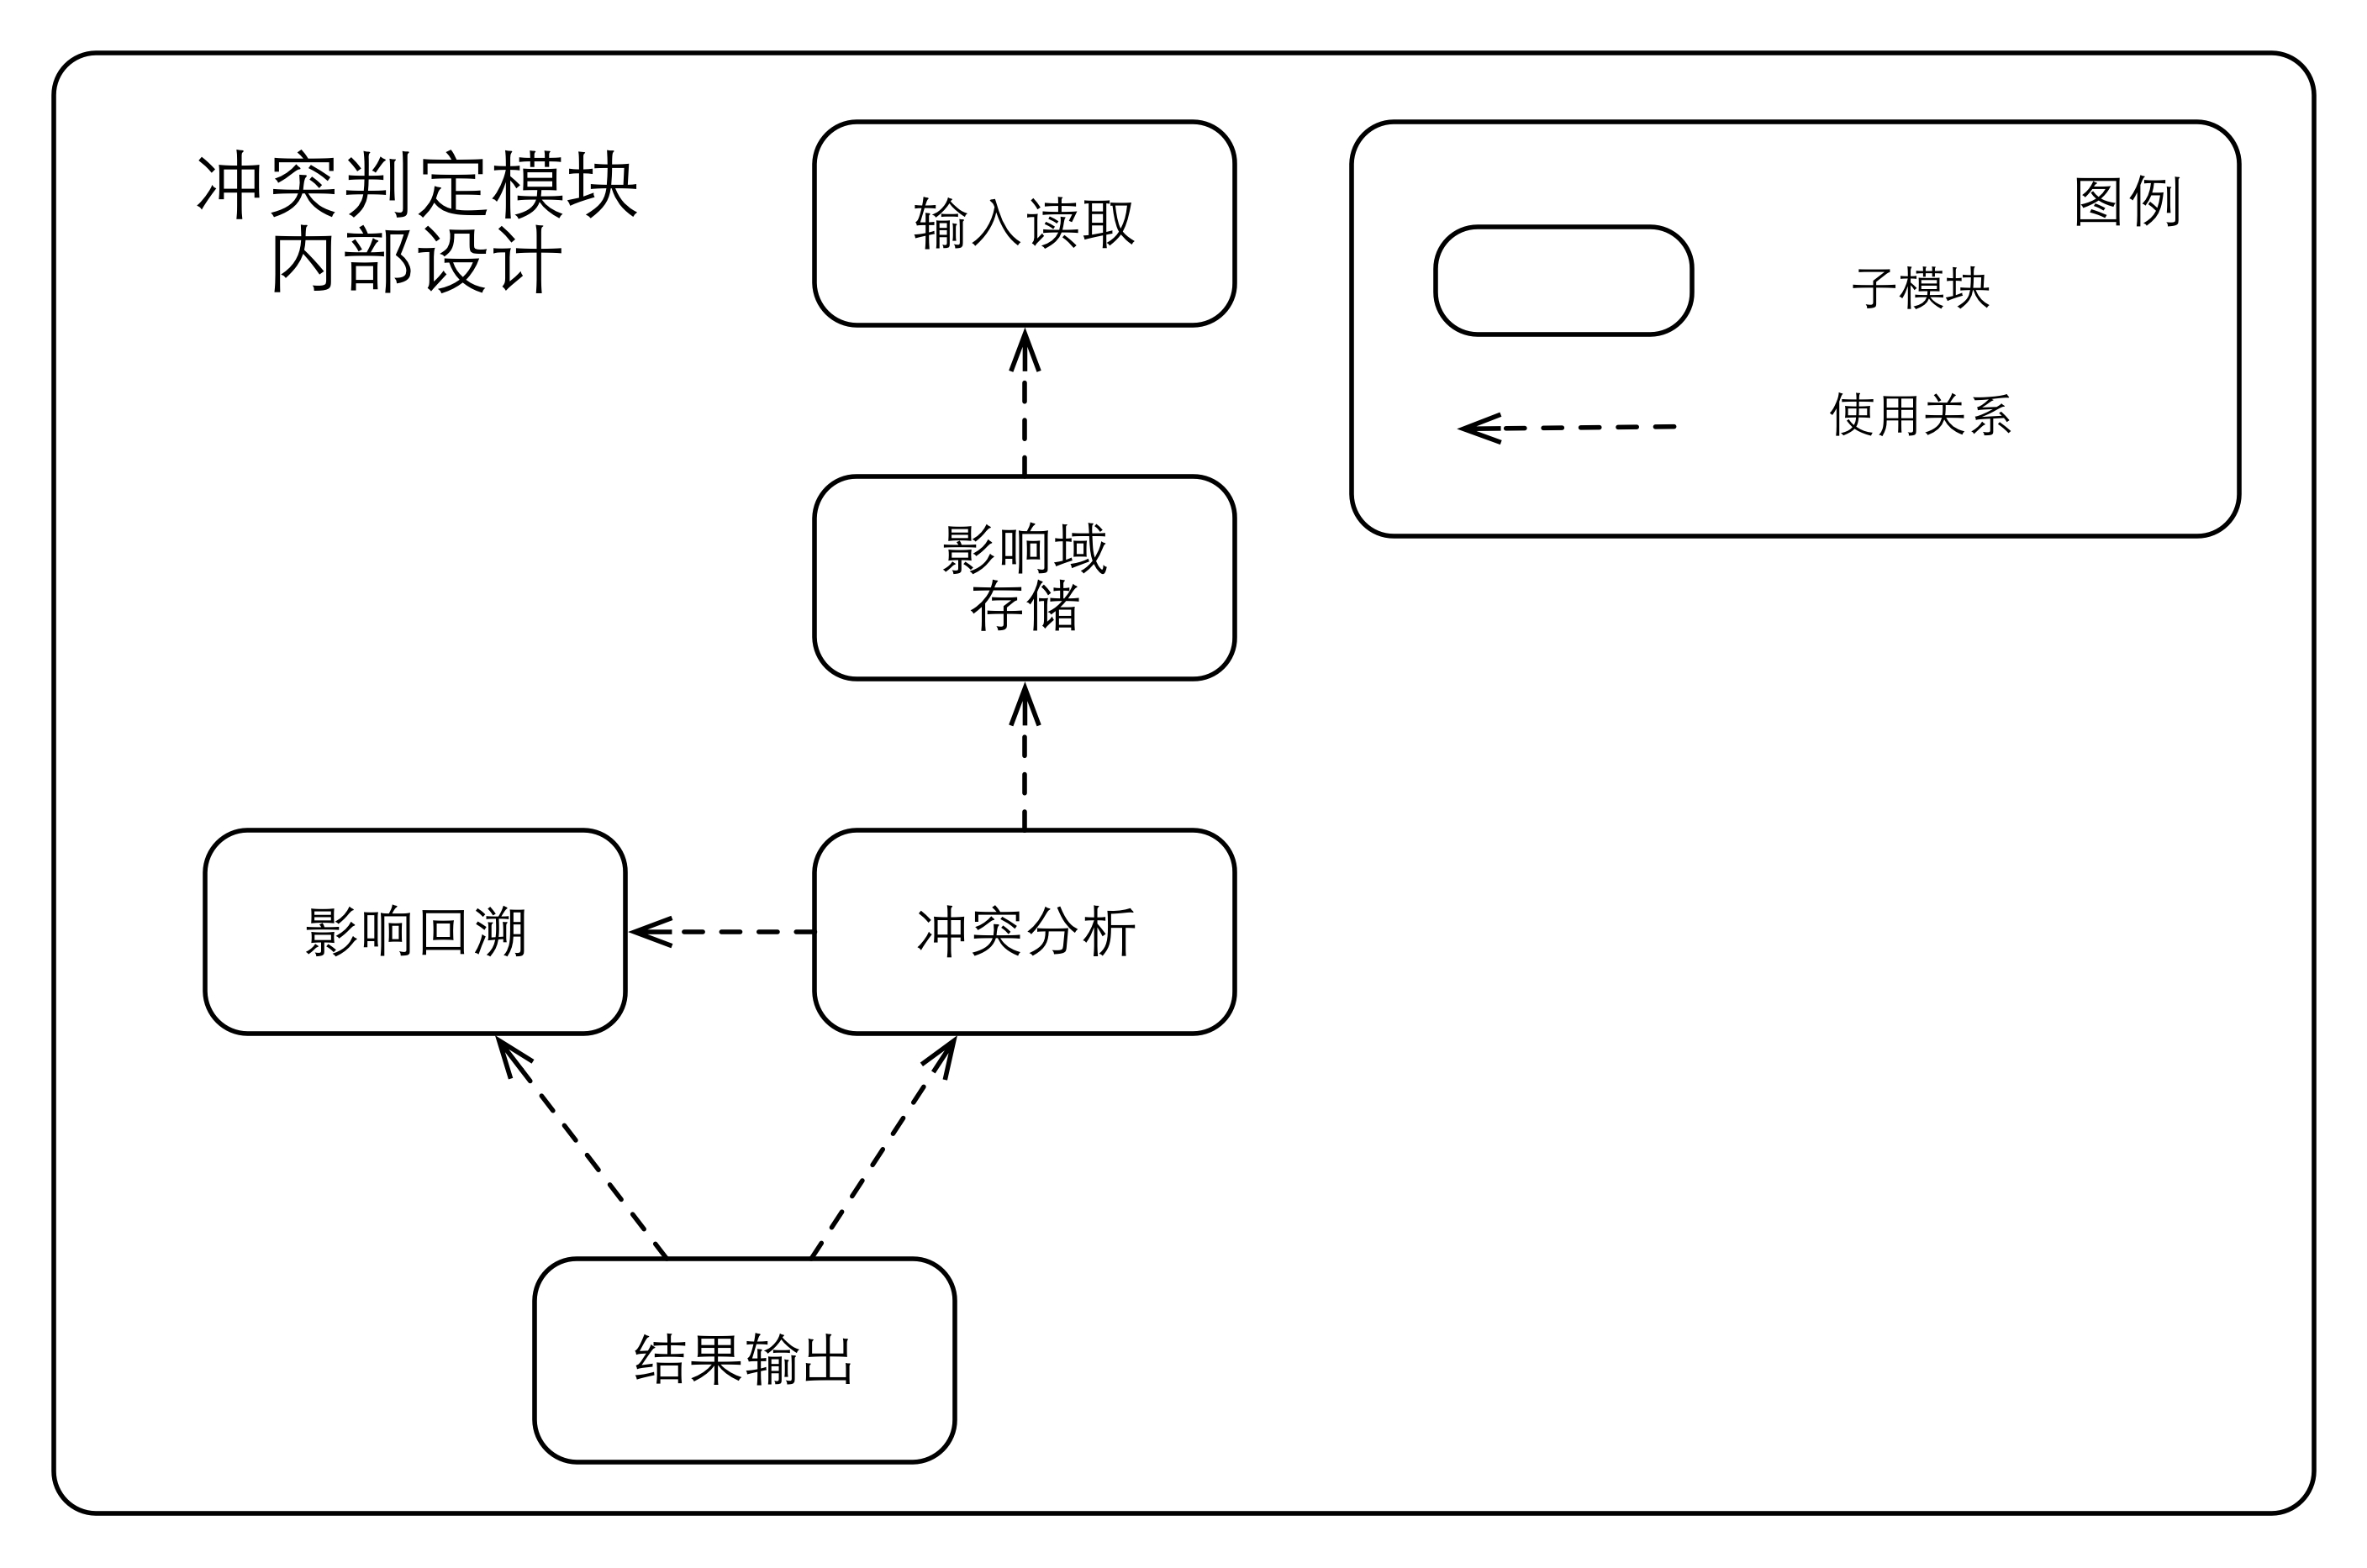
\includegraphics[width=.8\columnwidth]{chap04_com_internal}
%	\caption {模块设计}
%	\label {des_com}	
%\end{figure}
%
%\subsection{实现}

该模块的实现过程主要参考了算法\ref {algo_compatible}的描述。由于其输入为影响域模块的输出,因此它在输出时可以参照其输入给出类似形式的结果,即将重叠位置和其相关的影响关系作为额外的信息输出到控制流图中,以供人工分析使用。人工分析的过程主要是参考输出的部分控制流中,被标注为可能发生冲突的节点是否确实发生了冲突。

%在实际的实现中,其输入输出可以参考表\ref {com_io2}。

%\begin{table}[H]
%	\caption{输入输出对照表}
%	\label{com_io2}
%	\centering
%	\begin{tabular}{llc}
%		\toprule[1.5pt]
%		{\heiti 输入输出} & {\heiti 描述} & {\heiti 格式}\\\midrule[1pt]
%		输入 & $diff(v_2,v_1)$对于$v_2$的语义影响域 & Dot\\
%		输入 & $diff(v_2,v_4)$对于$v_2$的语义影响域 & Dot\\
%		输出 & 语义冲突 & Dot \\
%		\bottomrule[1.5pt]
%	\end{tabular}
%\end{table}

%可见,冲突判定模块中的主要工作包括:
%\begin{itemize}
%	\item 计算影响域的重叠
%	\item 对找到的语义冲突进行影响回溯,并以Dot格式将其涉及到的部分控制流和相关的冲突信息进行输出。
%\end{itemize}

冲突判定模块中的类实现可以参考图\ref {diff}。其中impactSet类用于存储影响域,DotNode和DotEdge用于存储从Dot文件中读取到的节点和边的信息,这两个类采用了多态机制来存储节点和边的类型信息。Diff类是从Dot文件中读取影响域并计算其重叠与否的类。相关的数据结构说明参考表\ref {diff_data}。

\begin{table}[H]
	\caption{Diff数据结构}
	\label{diff_data}
	\centering
	\begin{tabular}{lllc}
		\toprule[1.5pt]
		{\heiti 数据类型} &{\heiti 数据结构} & {\heiti 用途} \\\midrule[1pt]
		static void & main(String[] args) & 实现冲突分析过程\\
		void & analyzeDot(String path, impactSet now) & 读取Dot文件,将影响域存储于now \\
		void & readFileName(String path) & 读取待分析的文件名\\
		void & deleteDot(String p) & 删除输出\\
		void & computeImpact(impactSet s,impactSet s1) & 计算重叠\\
		void & output(Set<Integer> intersection, impact now) & 输出冲突和相关控制流\\
		void & printNode(BufferedWriter writer, DotNode node...) & 写控制流节点\\
		void &  WriteEdge(Set<Integer>  impacted...) & 写控制流边\\
		\bottomrule[1.5pt] 
	\end{tabular}
\end{table}

\begin{table}[H]
	\caption{impactSet数据结构}
	\label{impact_data}
	\centering
	\begin{tabular}{lllc}
		\toprule[1.5pt]
		{\heiti 数据类型} &{\heiti 数据结构} & {\heiti 用途} \\\midrule[1pt]
		String     &  path & 该影响域对应Dot文件的位置 \\
		Set<Integer>  &  allLoc & 存储影响域中的元素 \\
		Set<DotNode>  & nodes & Dot文件中的控制流节点\\
		Set<DotEdge>  & edges & Dot文件中的控制流边\\
		Map<Integer, Set<Integer>> & lineToNodeId & 从控制流边到节点ID的映射\\
		Map<Integer, DotNode>  & idToNode & 从节点ID到节点的映射 \\
		Map<Integer, Set<DotEdge>>  &  relation & 从节点ID到边的映射 \\
		\bottomrule[1.5pt] 
	\end{tabular}
\end{table}

\begin{table}[H]
	\caption{DotNode数据结构}
	\label{node_data}
	\centering
	\begin{tabular}{lllc}
		\toprule[1.5pt]
		{\heiti 数据类型} &{\heiti 数据结构} & {\heiti 用途} \\\midrule[1pt]
		Integer    &   begin & 该基本块的起始行号 \\
		Integer    &   end  & 该基本块的结束行号 \\
		Integer    & id & 该节点的ID \\
		boolean    & changed & 该节点是否属于变更集合 \\
		\bottomrule[1.5pt] 
	\end{tabular}
\end{table}

\begin{table}[H]
	\caption{DotEdge数据结构}
	\label{edge_data}
	\centering
	\begin{tabular}{lllc}
		\toprule[1.5pt]
		{\heiti 数据类型} &{\heiti 数据结构} & {\heiti 用途} \\\midrule[1pt]
		Integer   & begin & 该边的起始节点 \\
		Integer  &   end & 该边的结束节点 \\
		\bottomrule[1.5pt] 
	\end{tabular}
\end{table}

\begin{figure}[H]
	\centering
	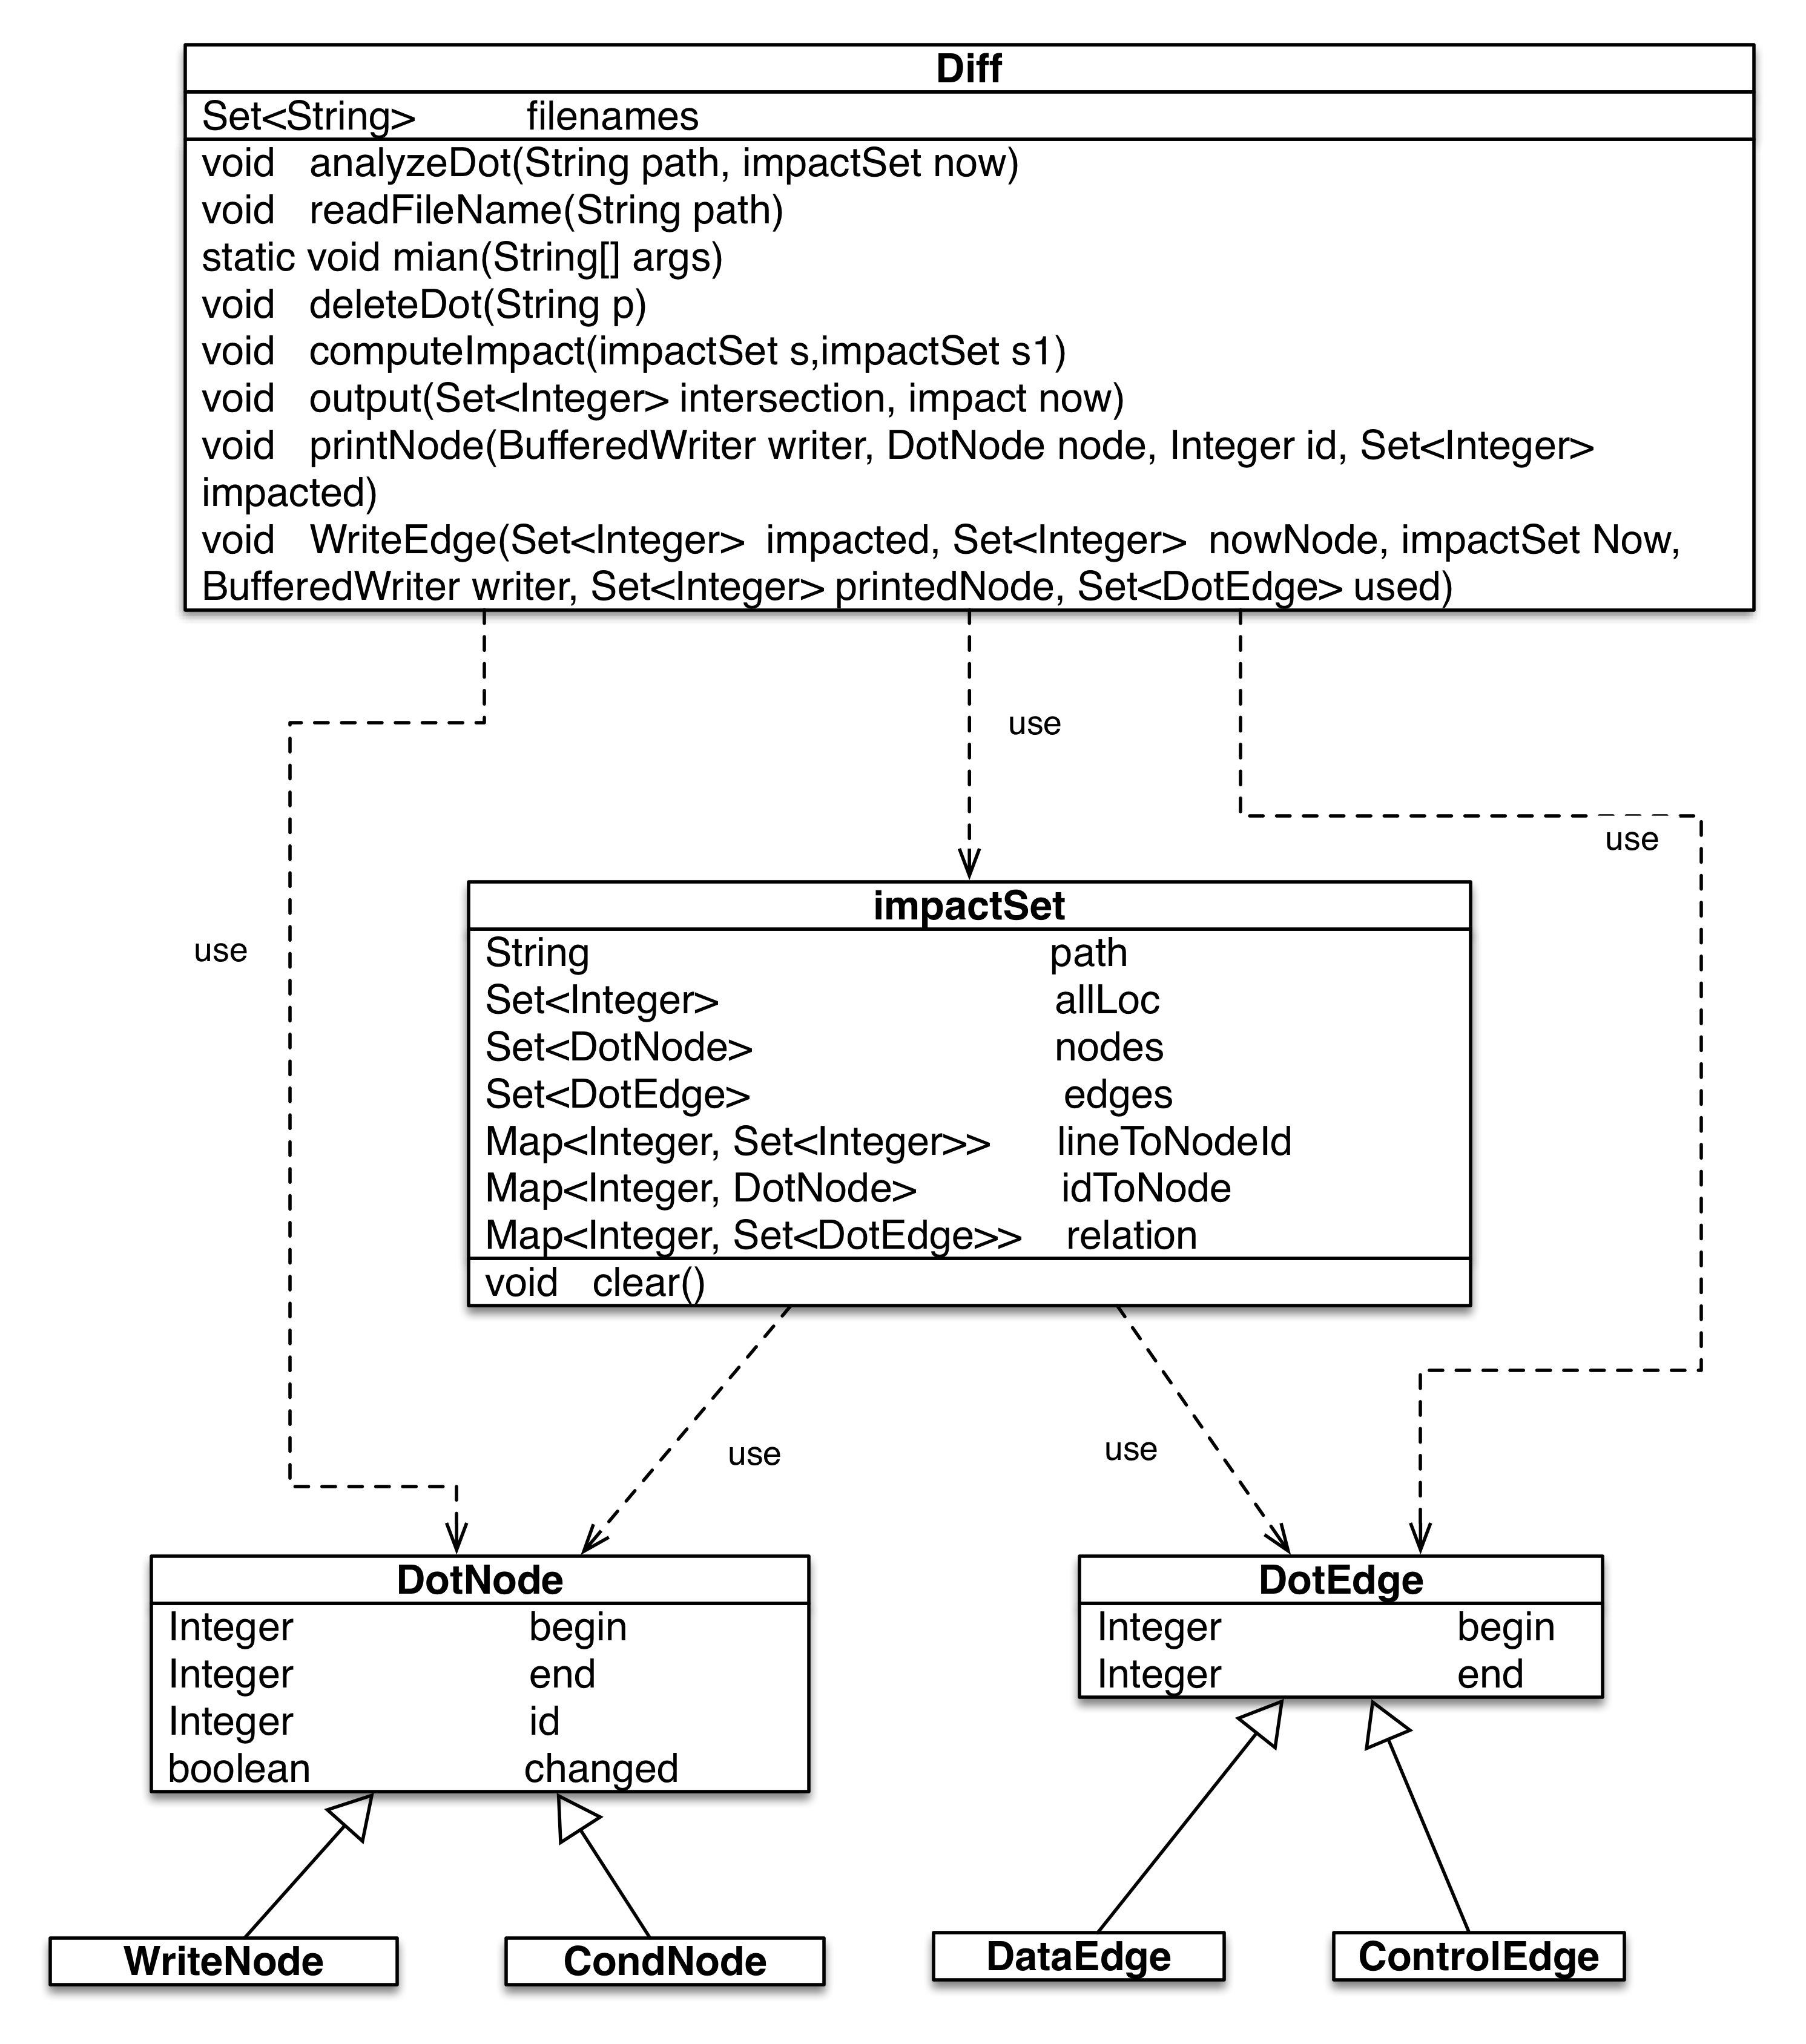
\includegraphics[width=.8\columnwidth]{chap04_diff}
	\caption {Diff类族}
	\label {diff}	
\end{figure}

综上所述,该模块的实际工作流程可以参考图\ref {com_flow}。

\begin{figure}[H]
	\centering
	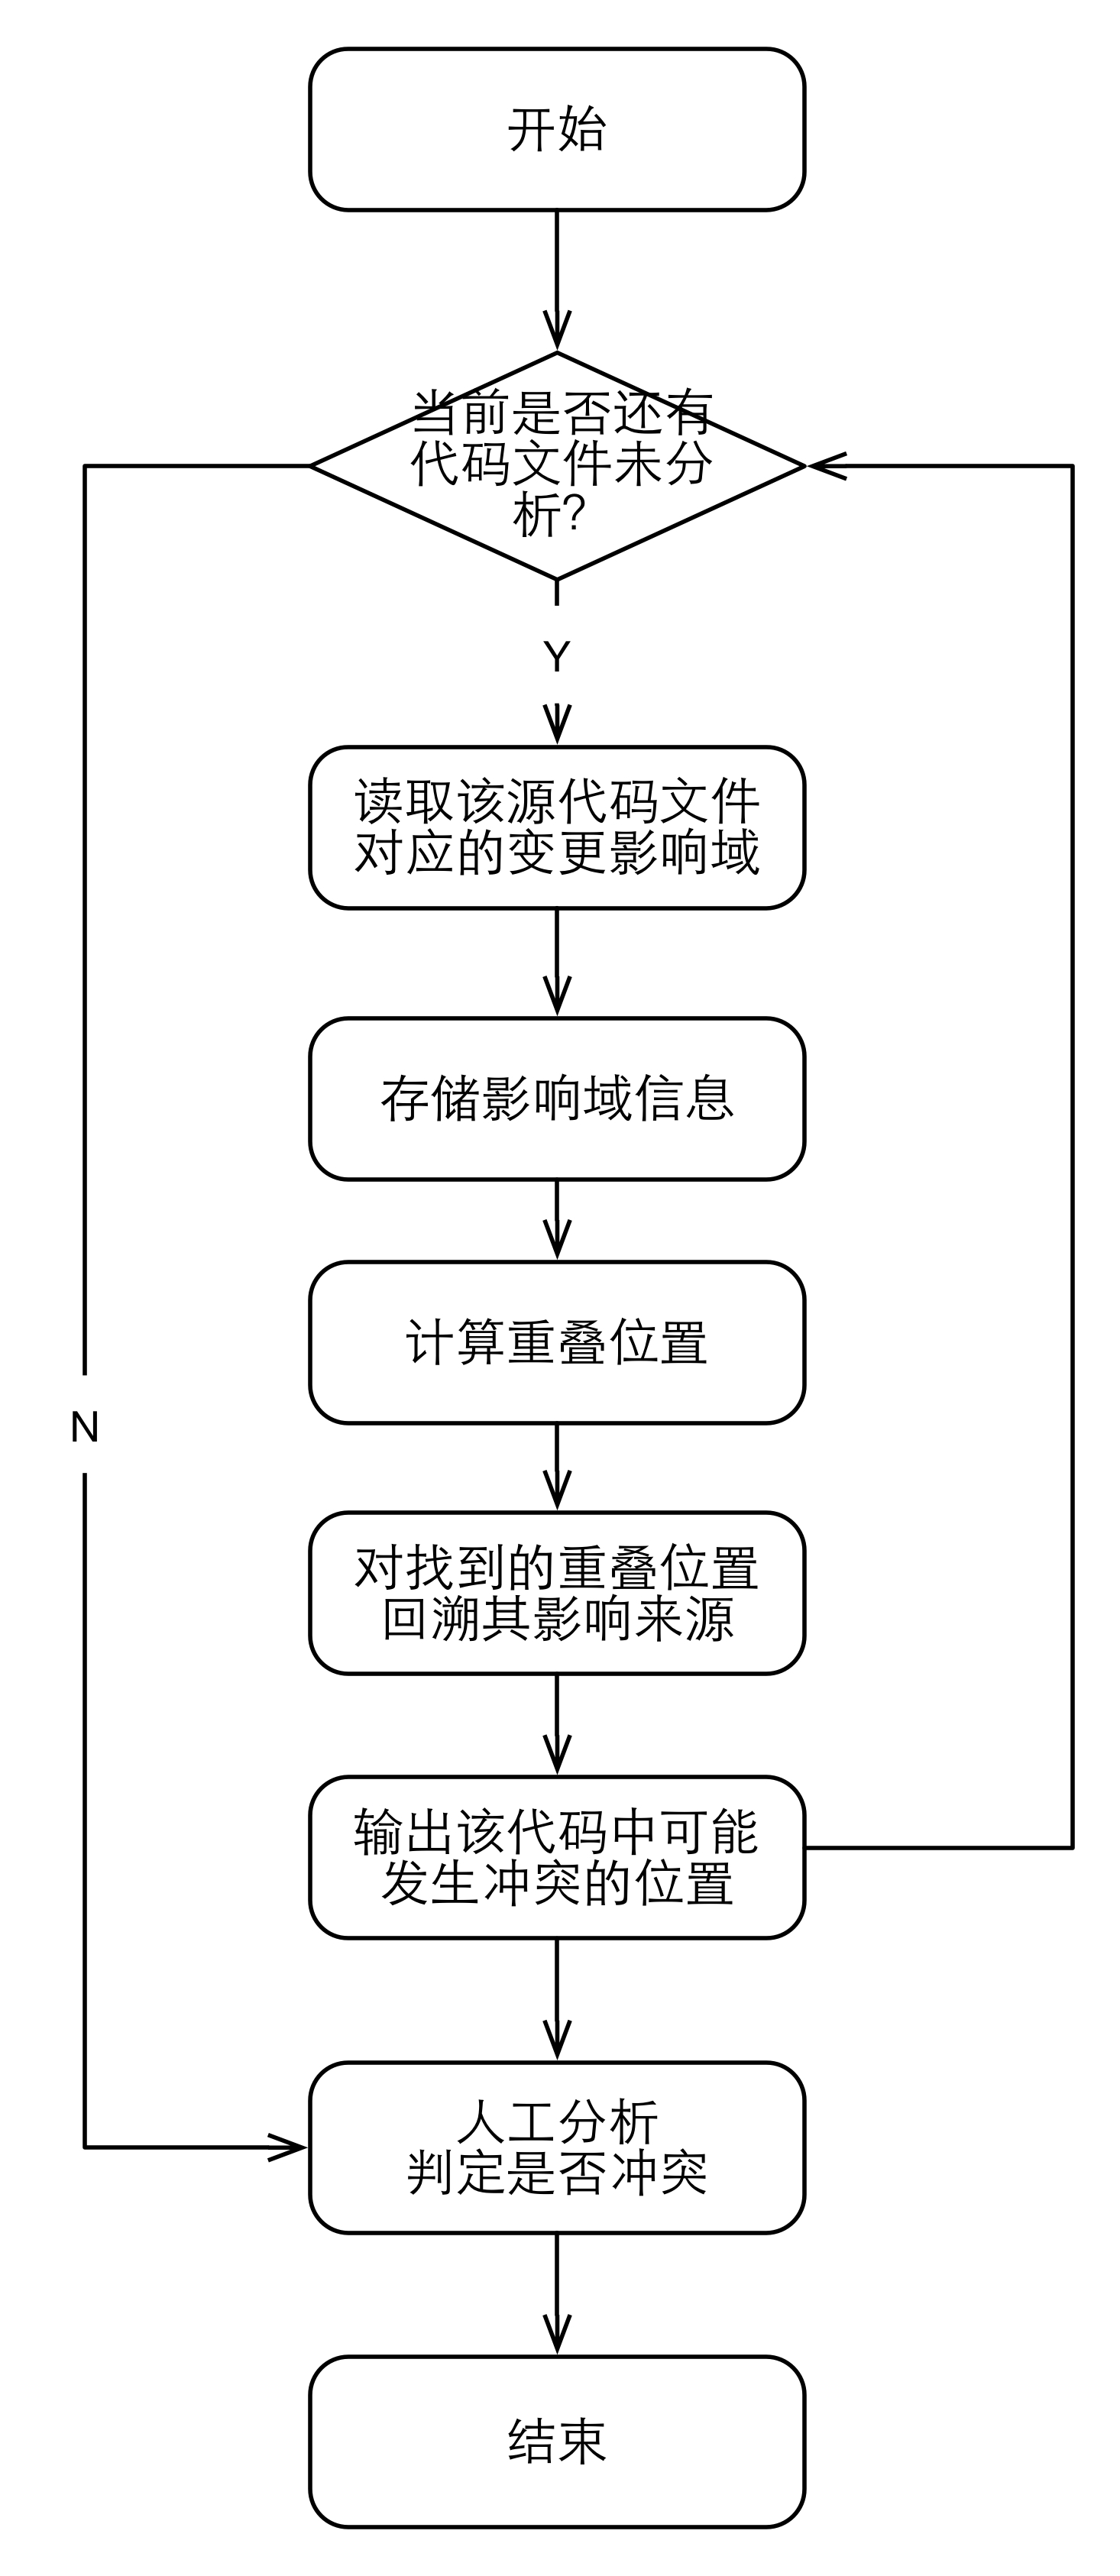
\includegraphics[height=.8\columnwidth]{chap04_com_flow}
	\caption {冲突检测模块流程}
	\label {com_flow}	
\end{figure}

\section{本章小结}

本章中主要介绍了软件变更冲突检测方法和其对应的模块设计与实现。
章节\ref {conflict_define}中介绍了冲突检测方法的相关定义。
章节\ref {chap_conflict}中介绍了冲突检测方法和其算法描述。
章节\ref {chap_mod}中介绍了冲突检测方法对应的工具模块其设计与实现。